\chapter{Anwendung}
\label{sec:Anwendung}

\section{Frameworks}
Die Anforderung an diese Seminararbeit war, dass Hibernate genutzt wird.
Zusätzlich habe ich mich mit Spring auseinandergesetzt. Speziell nutzte ich für diese Arbeit Spring MVC und Spring Data. Um die Darstellung der Web Oberfläche einfach und ansprechend zu gestalten habe ich Bootstrap \cite{Bootstrap} benutzt.

\section{Architektur}
Die Anwendung Besteht aus einer Webapplikation. Ich habe ein Model-View-Controller Ansatz gewählt wlecher mit dem Framework Spring MVC umgesetzt wurde. Web Anfragen werden von Spring entgegengenommen und an die Controller Klassen weitergeleitet, welche die Anfrage bearbeiten. Für das ORM habe ich Spring Data JPA und Hibernate verwendet.

\subsection{Dependencies}
Ich habe ein Maven Projekt gemacht, weshalt sämtliche Dependencies im pom.xml hinterlegt wurden.

\subsection{Struktur}
Der Source Code ist grundsätzlich in 3 Ordern untergebracht:
\begin{itemize}
	\item \emph{java}: hier sind sämtliche JAVA Klassen in verschiedenen Paketen untergebracht.
	\item \emph{resources}: hier werden Konfigurationsdateien gespeichert
	\item \emph{webapp}: hier sind die für die Web Applikation benötigten Dateien (jsp, css, js) und das web.xml gespeichert
\end{itemize}

\subsubsection{Pakete}
Ich habe für die Anwendung den Paket Prefix ch.zhaw.schilram genutzt. Die Anwendung hat den Namen sem\_hib. Die JAVA Klassen sind in verschiedene Pakete unterteilt.
\begin{figure}[h]
\centering
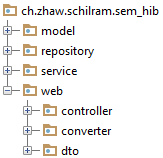
\includegraphics[width=0.2\columnwidth]{graphics/pakete.png}%
	\caption{Paketstruktur}
	\label{fig:Paketstruktur}
\end{figure}
\\
\textbf{model}\\
Im Paket \emph{model} sind die Model Klassen untergebracht welche von Hibernate für das ORM Mapping genutzt werden.\\\\
\textbf{repository}\\
Im Paket \emph{repository} sind sämtliche Sämtliche Interfaces welche das JPARepository Interface implementieren und für den Zugriff auf die Datenbank dienen.\\\\
\textbf{service}\\
Das Paket \emph{service} beinhaltet für jede Model Klasse eine Service Klasse welche die Methoden für den Zugriff auf die Datenbank ermöglicht.\\\\
\textbf{web.controller}\\
Im Paket \emph{web.controller} sind die Controller Klassen abgelegt welche die Web Requests entgegennehmen und verarbeiten\\\\
\textbf{web.converter}\\
Hier sind einerseits die Converter Klassen gespeichert, welche statische Methoden zur Umwandlung einer Model Klasse in die entsprechende DTO Klasse anbieten, sowie auch die Converter, welche gebraucht werden um über in Web Formularen als String übermittelte ID das zugehörige persistierte Objekts zu finden.\\\\
\textbf{web.dto}\\
Im Pakte \emph{web.dto} sind die DTO bzw. Formular Klassen welche für die Formulareingabe genutzt werden abgelegt.

\subsection{Klassendiagramm}
Unten sind die Klassendiagramme der Pakete \emph{model} und \emph{service} aufgeführt.

\subsection{model Klassendiagramm}

\begin{figure}[h]
\centering
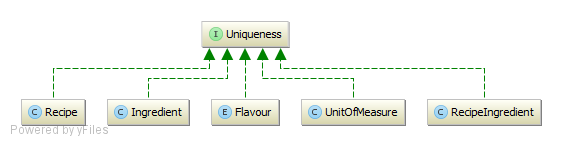
\includegraphics[width=0.6\columnwidth]{graphics/model_Klassendiagramm.png}%
	\caption{Klassendiagramm Paket \emph{model}}
	\label{fig:model_Klassendiagramm}
\end{figure}

\subsection{service Klassendiagramm}
\begin{figure}[h]
\centering
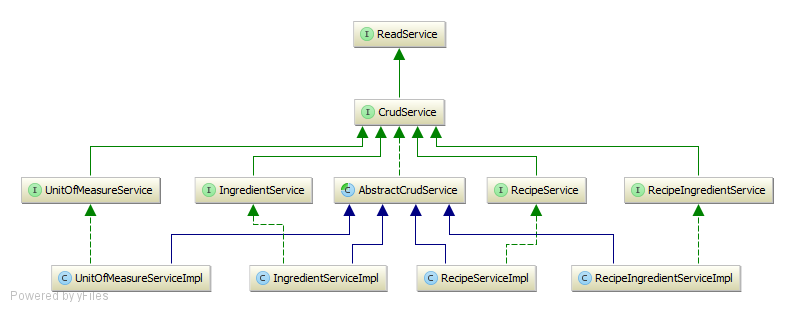
\includegraphics[width=0.6\columnwidth]{graphics/service_Klassendiagramm.png}%
	\caption{Klassendiagramm Paket \emph{service}}
	\label{fig:service_Klassendiagramm}
\end{figure}

\section{Installation}

\subsection{Voraussetzungen}
Damit die Applikation läuft muss sie auf eine Datenbank zugreifen können. Zusätzlich wird Tomcat vorausgsetzt um die Web Applikation laufen zu lassen.

\subsection{Datenbank einrichten}

CREATE ROLE sem_hib LOGIN ENCRYPTED PASSWORD 'md5198ad17e37731cbad30b3130a0a88919'
   VALID UNTIL 'infinity';
	
CREATE DATABASE sem_hib
  WITH ENCODING='UTF8'
       OWNER=sem_hib
       CONNECTION LIMIT=-1;

	
	

\subsection{Tomcat einrichten}


